% 20 Apr 2014 : GWA : 4 pages.

\section{Evaluation}
\label{sec-evaluation}

\begin{figure}[t]
  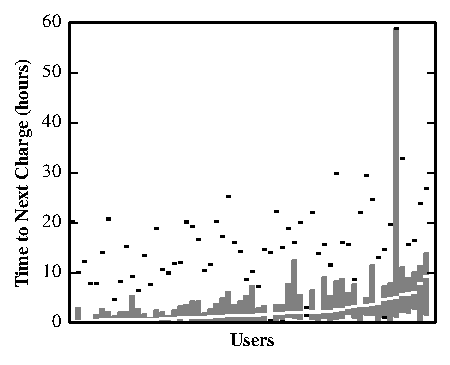
\includegraphics{./figures/pocketlocker/BatteryLengthDistributionGraph.pdf}
  
  \caption{\small \textbf{Time Until Next Charge After File Creation.}
    Separating the process of creating files into two steps allows
  PocketLocker to reduce energy consumption by performing transfers during
the next charging cycle.}
  
  \label{fig-simulation-battery}

  \vspace*{-0.2in}
\end{figure}

We evaluate PocketLocker in two ways. First, we analyze the file access
traces we collected on \PhoneLab{} to determine the impact of parameters
important to PocketLocker's design. We also use the traces as inputs to a
trace-based simulation to compare approaches to performing client storage
reclamation. Second, we perform detailed measurements of our PocketLocker
prototype engaging in the types of file accesses described previously.
Our results indicate how utilizing nearby clients can improve performance, and
also how PocketLocker enables energy-efficient operation on battery-powered
clients.

\subsection{Trace Analysis}
\label{subsec-evaluation-traces}

\begin{figure*}[t]
  \centering
  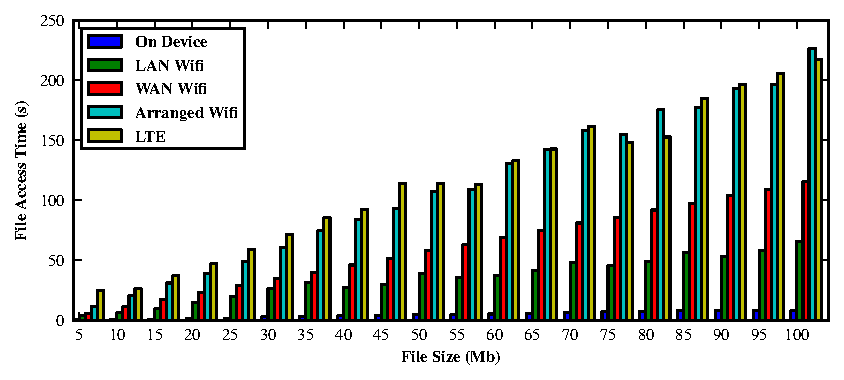
\includegraphics{./figures/downloadtimes.pdf}
  
  \vspace*{-0.1in}

  \caption{\small \textbf{PocketLocker file access times.} Figure
    illustrates the
    times required to access files of various sizes by PSC in different
    types of
  connectivity.}

  \label{fig-evaluation-download}
  
  \vspace*{0.05in}

  %\hrule

  \vspace*{-0.2in}

\end{figure*}

PocketLocker relies on nearby clients to improve performance of file accesses.
In the best case, other PSC clients are located on the same LAN. To determine
whether nearby clients can assist with file accesses, we performed further
analysis of the traces described in Section~\ref{sec-motivation}.

Because \PhoneLab{} only provides visibility into participant smartphones, we
have to infer where users would have other PSC clients nearby. To do so, we
simulated the presence of PocketLocker PSC clients on the two Wifi networks
that each user spent the most time connected to, which could represent home
and work networks. We then divided file accesses into three categories: (1)
ones that occur on the same LAN with a simulated PSC client, (2) those that
do not occur on a PSC LAN but still occur while the user is connected to a
high-speed and energy-efficient Wifi network, and (3) those that occur when
the user is connected to a mobile data network\footnote{We found no file
  accesses that occurred more than five minutes from log messages indicating
  the presence of a mobile data network, a reflection of the always-connected
nature of smartphones.}. Figure~\ref{fig-simulation-connectivity} shows the
results. For around half of the users, even without a local cache half of the
file accesses could be served by two clients placed at their most used Wifi
networks. Only in the remaining half of accesses, where files are not locatable
on another PSC client on the lan, must a device go outside the network.

We were also interested in how many file creations could be offloaded to
powered clients by delaying transfer until the user plugged their smartphone
in to charge. Figure~\ref{fig-simulation-battery} shows per-user
distributions of the of time between file creations and the next charging
session. For all users, the median is under 10~hours with worst-case maximums
approaching a day. Overall, the results suggest that by delaying the initial
file transfer required during creation for a portion of the user's backup
window, PocketLocker can enable energy-neutral transfers and reduce overhead
on battery-powered clients.


Finally, we built a trace-based simulator to experiment with different
policies for managing the mobile client chunk store. We configured each PSC
client smartphone with 1~GB of storage, considerably less than the amount of
file accesses we observed during our one-month experiment, and managed the
chunk store using four different algorithms: random eviction,
first-in-first-out (FIFO), least-recently-used (LRU), and least-accessed
first (Access). Figure~\ref{fig-simulation-policy} compares the results. When
file accesses missed the chunk store, we classified the access as described
previously based on the smartphone's connectivity at that moment.
Surprisingly, we did not observe any large performance differences between
these algorithms, although they were able to manage the local
chunk store to absorb a large number of file accesses. A great
deal of inter-user variation is visible, and we are continuing to study
how to better adapt PocketLocker's reclamation algorithms to the specifics of
each users file access patterns.
\begin{figure}[t]
  
  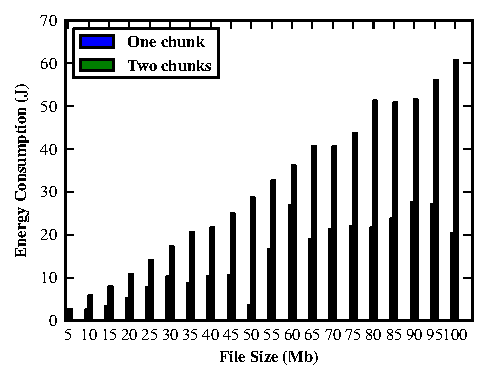
\includegraphics[scale=.97]{./figures/energysavings.pdf}
  
  \caption{\small \textbf{PocketLocker energy savings.} The figure
    illustrates the savings in energy when an interactive device downloads
  one chunk compared to downloading two chunks to access the file.}
  
  \label{fig-evaluation-energysavings}

  \vspace*{-0.2in}
\end{figure}

\subsection{Prototype Performance Evaluation}
\label{subsec-performance-evaluation}

We evaluated the prototype of the implementation described in
Section~\ref{sec-implementation} in two ways. First, we measured the time
required to access files of various sizes with devices connected to different
networks types. Secondly, we measured the energy consumption to access files.
In our experiments we chose $k=2$ as the number of chunks required for
reconstruction. We used Samsung Galaxy S4 and Nexus 5 smartphones as
interactive devices, and utilized Android VMs running PocketLocker as fixed
nearby devices.

\subsubsection{File access:\space} \label{sec-fileaccess}
Figure~\ref{fig-evaluation-download} illustrates the time required to download
files of different sizes with clients having to download $k$ chunks to
reconstruct the file when connected to different networks. The \textit{On
Device} scenario denotes the time required to reconstruct the original file
from the chunks that are available locally on the device. This is the best
scenario as there are no chunks downloaded from other sources. In \textit{LAN
  Wifi}, we
have a fixed device present on the same LAN as the interactive device. The
device downloads both the chunks required to reconstruct the file from the fixed
device and is the fastest compared
to any other connection type. \textit{WAN Wifi} has fixed devices that are
publicly accessible over the Internet to the interactive devices. WAN Wifi is
analogous to downloading files from the cloud today. \textit{Arranged Wifi}
presents the scenario where the fixed devices are not publicly accessible and
data transfers are done via a relay. As seen in
Figure~\ref{fig-evaluation-download}, the time to open a file when the
chunks are downloaded on the LAN Wifi are almost 50\% faster when compared to
WAN Wifi scenario. This result is encouraging, as we envision most chunk
transfers happening over LAN Wifi.

\subsubsection{Energy Consumption:\space}We used the Monsoon power
monitor~\cite{monsoon} to measure the energy consumption
for the scenarios described in Section~\ref{sec-fileaccess}.
Figure~\ref{fig-evaluation-energy} illustrates the average energy consumption
over five experiment runs on the
interactive device. As expected, data transfers over the cellular network
consumes the most amount of energy and the scenarios using the WiFi interface on
the interactive device consume significantly lesser energy compared to the
scenario where cellular network is used. Figure~\ref{fig-evaluation-energysavings}
compares the energy consumption of file access when downloading two chunks
with the energy required to access the file by downloading one chunk. The
energy consumption when accessing the file by downloading one
chunk is less than the consumption to access the file by downloading both
chunks. This is a positive result for PocketLocker as it stores only some of
the required chunks instead of all chunks under storage pressure.

Energy consumption by smartphones when pushing recently created file chunks to
remote storage does not pose a similar issue.  The System deliberately dictates
that devices wait until plugged in before they commence upload.

\subsection{Scalability:\space} The purpose of PocketLocker is to furnish a
mobile device-aware personal storage subsystem. Each user typically will have
on the order of tens of devices connected to the system, which can be easily
coordinated by the user's orchestrator. Thus, growth of the userbase encounters
no limit: each user has its own PSC supported by an individual instance of an
orchestrator.


\begin{figure*}[t]
  \centering
  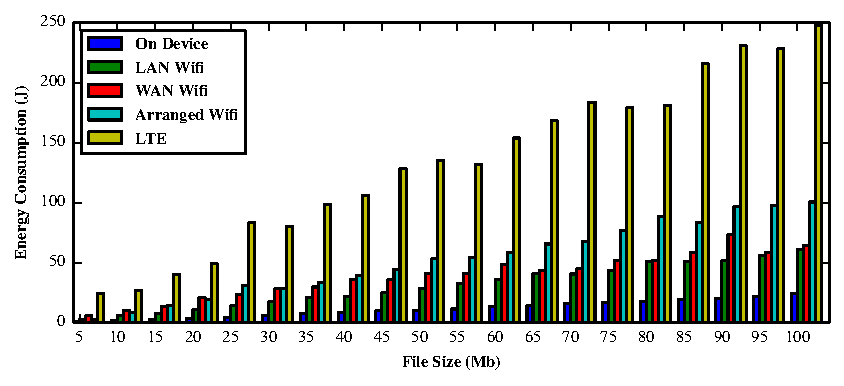
\includegraphics[width=0.8\textwidth]{./figures/energyconsumption.pdf}
  
  \vspace*{-0.1in}

  \caption{\small \textbf{PocketLocker energy consumption.}Figure illustrates the energy
  consumption on interactive device to access files of different sizes from
fixed devices in various types of network.}

  \label{fig-evaluation-energy}
  
  \vspace*{0.05in}

%  \hrule

  \vspace*{-0.2in}

\end{figure*}


